\chapter*{Anexos}
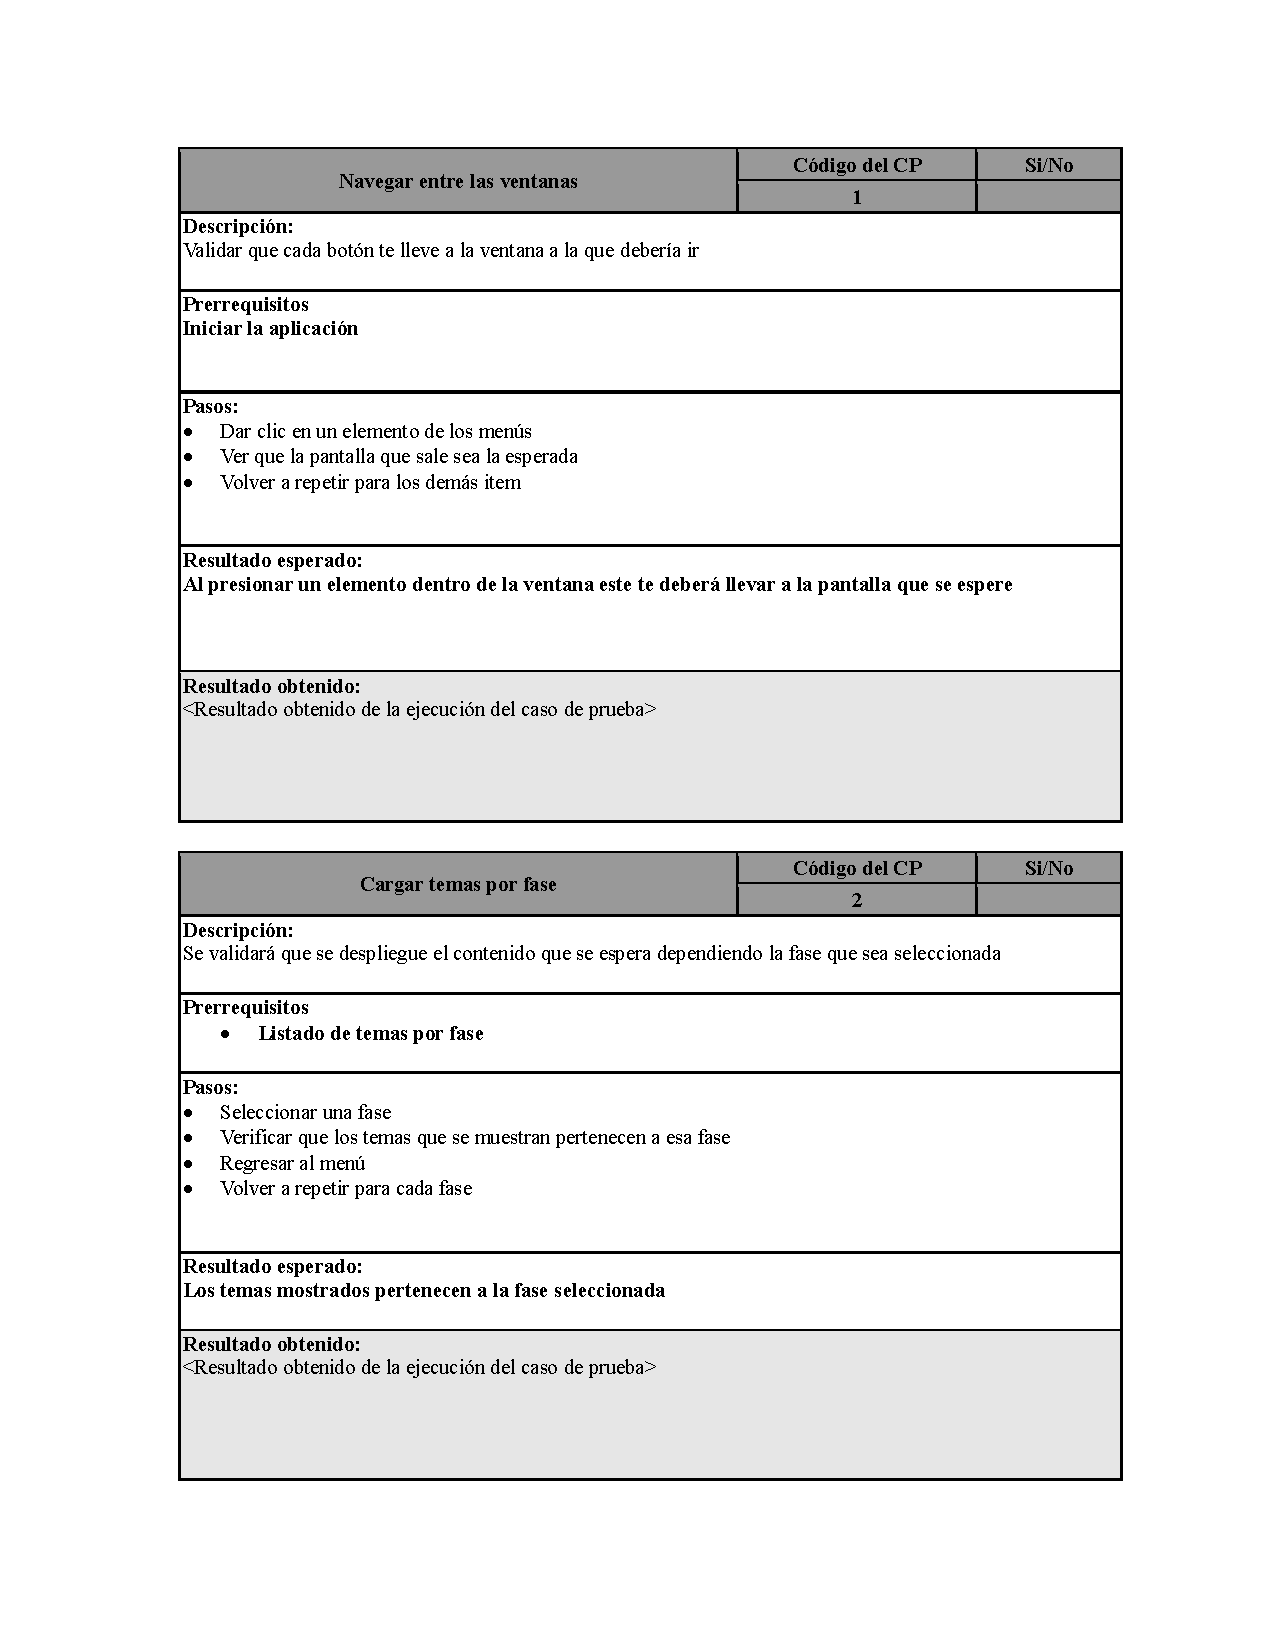
\includepdf[pages=-]{cdp}

\begin{table}[H]\small
\begin{tabular}{@{\extracolsep{\fill}} |p{9cm}|p{4cm}|p{2cm}|}
\hline
\textbf{1. Navegar entre las ventanas} & \textbf{Código del CP:} & \textbf{Si / No} \\ \hline
\multicolumn{3}{|p{15cm}|}{\textbf{Descripción:}

Validar que e botón te lleve a la ventana que debería ir.} \\ \hline
\multicolumn{3}{|p{15cm}|}{Prerequisitos:

Iniciar la aplicación.} \\ \hline
\multicolumn{3}{|p{15cm}|}{\textbf{Pasos:}
\begin{itemize}
	\item Dar click en un elemento de los menús.
	\item Ver que la pantalla que sale sea la esperada.
	\item Volver a repetir para los demás item
\end{itemize}}\\ \hline
\multicolumn{3}{|p{15cm}|}{\textbf{Resultado esperado:}

Al presionar un elemento dentro de la ventana este te deberá llevar a la pantalla que se espere.} \\ \hline
\multicolumn{3}{|p{15cm}|}{\textbf{Resultado obtenido:}

<Resultado esperado de la ejecucion de la prueba>} \\ \hline
\hline
\end{tabular}
\caption{Caso de prueba numero 1}
\label{p1}
\end{table}